\documentclass[11pt, a4paper]{article}
\usepackage[utf8x]{inputenc}
\usepackage[sort]{natbib}
\usepackage[linktoc=all]{hyperref}

\usepackage[spanish]{babel}
\usepackage{enumitem}
\usepackage{graphicx}
\usepackage{float}

\usepackage{etoolbox}

\usepackage{amsmath}
\usepackage{array}
\usepackage{gensymb}

\usepackage{fancyhdr}
\usepackage{multirow}
\usepackage{multicol}
\usepackage[table]{xcolor}
\usepackage{color}
\usepackage{colortbl}
\definecolor{lightgray}{gray}{0.9}
\setlength{\columnsep}{0.5cm}

\usepackage{tikz}
\usetikzlibrary{shapes.geometric, arrows}
\tikzstyle{problema} = [rectangle, rounded corners,  minimum width=3cm, minimum height=1cm,text centered, draw=black,fill={rgb:black,1;white,30}]
\tikzstyle{causa} = [rectangle, minimum width=3cm, minimum height=1cm, text centered, text width=4cm, draw=black, fill={rgb:black,0;white,10}]
\tikzstyle{nodo} = [diamond, minimum width=1cm, minimum height=1cm, text centered, draw=black, fill={rgb:black,0;white,10}]
\tikzstyle{arrow} = [thick,->,>=stealth]

%------------------- Dimensiones -------------------
\usepackage{geometry}
 \geometry{a4paper,total={170mm,257mm},left=15mm,right=15mm,top=20mm,}
%----------------------------------------------------

%------------------- Encabezado y Pie de pág -------------------
\pagestyle{fancy}
\fancyhf{}
\lhead{Electrónica de Potencia}
\rhead{TP6 : Inversor trifásico $SPWM$}
\rfoot{Página \thepage}
%----------------------------------------------------

%----------------------------- Documento -----------------------------------------------
\begin{document}
\begin{titlepage}
 \centering
	
\includegraphics[scale=0.80]{Imagen/LOGO.jpg} \par
 	\vspace{1cm}
 	{\scshape\LARGE Universidad Tecnológica Nacional \par}
 	{\scshape\large Facultad Regional de Córdoba \par}
 	\vspace{1cm}
	{\bfseries \Large Trabajo Práctico De Laboratorio $N^{\circ} 6$\par}
	{\bfseries \Large Diseño de un inversor trifásico $SPWM$ \par}
 	\vspace{1.5cm}

	\begin{tabular}{ll}
		Alassia, Francisco		&	60861	\\
		Amaya, Matías			&	68284	\\
		Lamas, Matías			&	65536 	\\
		Navarro, Facundo		&	63809 	\\
		Veron, Misael			&	62628
	\end{tabular}
	
	\vspace{1cm}
	Curso: 5r2 \\
	Grupo $N^{\circ} 11$
 	\vfill
	{\bfseries \Large Electrónica de Potencia \par}

	\vspace{1.5cm}
	Docentes: \par
	Ing. Oros, Ramón \par
	Ing. Avramovich, Javier \par

 	\vfill
	{\large \today\par}
\end{titlepage}
	
	
	\tableofcontents

%----------------your title below -----------------------------

\section{Introducción}
En el presente trabajo se estudia el diseño y funcionamiento, a partir de su simulación, de un inversor trifásico con técnica SPWM en lazo abierto con técnica de modulación SPWM trifásica unipolar y una línea de alimentación de 380 $V_{RMS}$ trifásica, 50 Hz.


El circuito de potencia de un inversor trifásico consta de seis interruptores controlables. La idea detrás de SPWM es generar el patrón de conmutación de los seis elementos de potencia. Este patrón se obtiene a partir de la comparación de una señal triangular de frecuencia y amplitud fijas (portadora) con una señal senoidal de frecuencia y amplitud variables (moduladora), tal como se observa en la Fig \ref{fig:spwm}.

\begin{figure}[h]
	\centering
	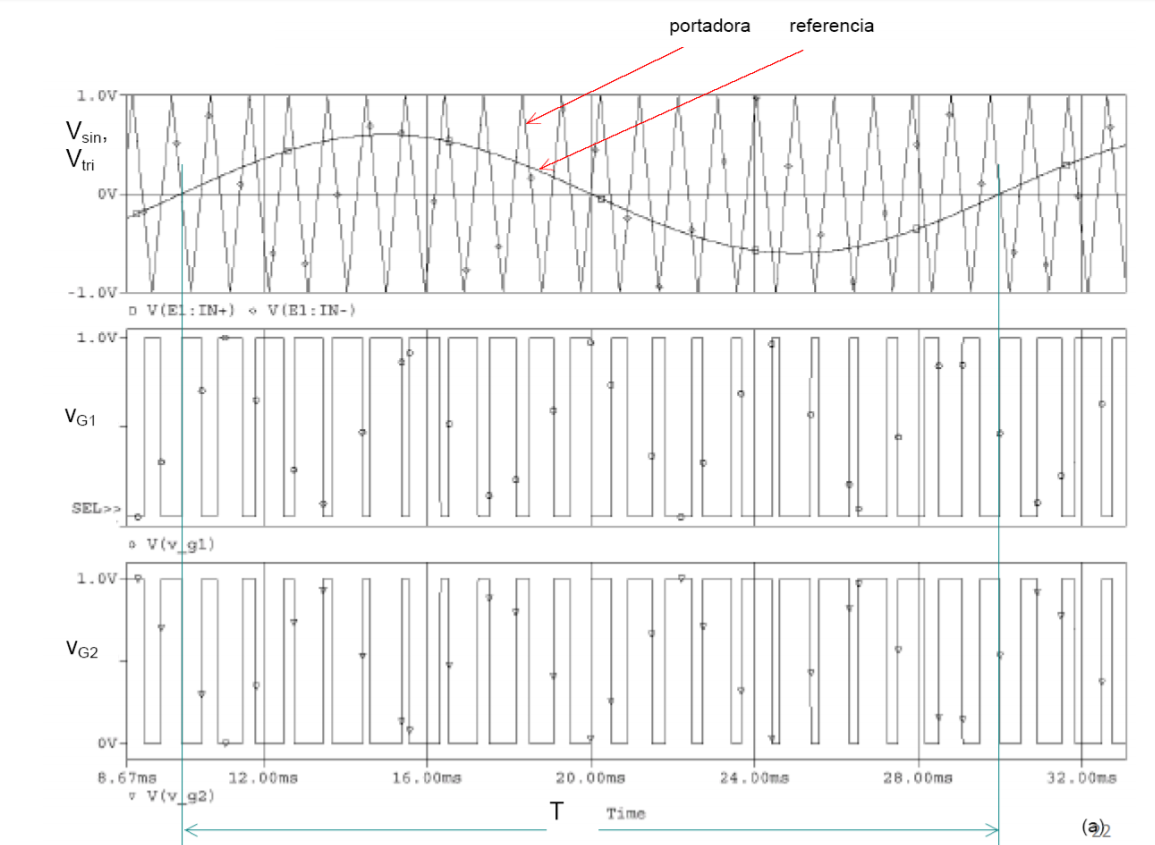
\includegraphics[width=15cm]{Imagen/SPWM}
	\caption{Patrón generado por la técnica SPWM.}
	\label{fig:spwm}
\end{figure} 

\section{Enunciado}
\begin{enumerate}
	\item Diseñar y simular un inversor trifásico SPWM en lazo abierto. Especificaciones:
	\begin{enumerate}
		\item Técnica de modulación SPWM trifásica unipolar.
		\item Línea de alimentación: 380 $V_{RMS}$ trifásica, 50 Hz.
		\item Frecuencia de salida del inversor variable de 2 a 200 Hz, controlable por un mando de frecuencia de referencia.
		\item Tensión de salida variable y controlable por un mando de tensión de referencia.
		\item Las referencias de frecuencia y tensión deberán ser controles al inversor independientes.
	\end{enumerate}
	\item Efectuar las siguientes mediciones:
	\begin{enumerate}
		\item Tensión de salida en cada fase, para tres mandos distintos de tensión y frecuencia de referencia.
		\item Espectro de frecuencia de la tensión de salida.
	\end{enumerate}
\end{enumerate}

\section{Marco Teórico}
\subsection{Generalidades}
La función del inversor es la de cambiar la tensión de entrada de CC en una tensión simétrica de salida CA con una magnitud, frecuencia y fase deseada. Un inversor, en definitiva, es un convertidor que transfiere potencia desde una fuente de continua a una carga de alterna. 

Un inversor básico consta de un transistor controlado por un oscilador, cuya función es interrumpir la corriente entrante y generar una onda cuadrada. Esta onda cuadrada alimenta a un transformador que suaviza su forma, haciéndola parecerse un poco mas a una onda senoidal y produciendo el voltaje de salida necesario. Debido a que se busca una tensión de salida alterna, las formas de onda de salida del voltaje de un inversor ideal deberían ser sinusoidales. Una buena técnica para lograr esto es utilizar PWM, consiguiendo que la componente principal senoidal sea mucho más grande que las armónicas superiores.

En los inversores senoidales reales, la salida no es senoidal pura, por lo que contiene ciertos armónicos. Para aplicaciones de baja y mediana potencia, se pueden aceptar tensiones cuadradas o casi cuadradas en lugar de la senoidal (ideal). Pero para aplicaciones de alta potencia, son necesarias las formas de onda senoidales de baja distorsión. 
Con la disponibilidad actual de dispositivos de conmutación de alta velocidad y potencia, y con la técnica de modulación adecuada, es posible disminuir significativamente el contenido armónico en la tensión de salida.

Los inversores se utilizan en una gran variedad de aplicaciones, desde pequeñas fuentes de alimentación para computadoras, hasta aplicaciones industriales para controlar alta potencia. También se utilizan para convertir la corriente continua generada por los paneles solares fotovoltaicos, acumuladores o baterías, etc., en corriente alterna y de esta manera poder ser suministrada en la red eléctrica o usada en instalaciones eléctricas aisladas.

\subsection{Parámetros de Rendimiento}
La calidad de un inversor se evalúa en función de los siguientes parámetros de rendimiento.
\subsubsection{Factor armónico de la enésima componente $HF_n$}
Es una medida de la contribución individual de la enésima armónica. $V_1$ es el valor RMS de la componente fundamental y $V_n$ el valor RMS de la componente enésima.
\[ HF_n = \frac{V_n}{V_1} \]

\subsubsection{Distorsión armónica total $THD$}
Es una medida de la similitud entre la forma de onda y su componente fundamental. Idealmente, debería ser 0\%. Si se supone que no hay componente de continua, se puede definir como:

\[ THD_V = \frac{\sqrt{\sum_{n=2,3,..}^{\infty} Vn^{2}_{RMS}}}{V1_{RMS}} = \frac{\sqrt{V^{2}_{RMS} - V1^{2}_{RMS}}}{V1_{RMS}} \]

\[ THD_I = \frac{\sqrt{\sum_{n=2,3,..}^{\infty} in^{2}_{RMS}}}{i1_{RMS}} = \frac{\sqrt{i^{2}_{RMS} - i1^{2}_{RMS}}}{i1_{RMS}} \]


\subsubsection{Factor de distorsión $DF$}
Proporciona el contenido armónico total, pero no especifica el nivel de cada uno de sus componentes. Si en la salida de los inversores se utiliza un filtro, las armónicas de orden más alto se atenuarán con mayor eficacia. Por lo tanto, resulta importante conocer tanto la frecuencia como la magnitud de cada componente. 

El factor de distorsión indica la cantidad de distorsión armónica que queda en una forma de onda particular después de que las armónicas de esa forma de onda hayan sido sujetas a una atenuación de segundo orden (es decir, divididos por $n^2$).

El valor de $DF$ es una medida de la eficacia en la reducción de las componentes armónicas no deseadas, sin necesidad de especificar valores de un filtro de carga de segundo orden, y se define como:

\[ DF = \frac{1}{V_1} \cdot \sqrt{\sum_{n=2,3,..}^{\infty} (\frac{V_n}{n^{2}})^{2}} \]

El $DF$ de la componente armónica individual o de orden n, se define como:

\[ DF = \frac{V_n}{V_1 \cdot n^2} \]

\subsubsection{Armónica de menor orden $LOH$}
Es aquella componente cuya frecuencia es más cercana a la fundamental y cuya amplitud es mayor o igual que el 3\% de la fundamental.

\subsection{Inversor Trifásico}
Pueden ser vistos como tres convertidores monofásicos conectados entre sí, que se utilizan en aplicaciones de alta potencia. Las señales de compuerta o de base de los transistores deben adelantarse o atrasarse 120° uno respecto de otro con el fin de obtener voltajes trifásicos equilibrados. 

Los bobinados primarios del transformador deben estar asilados entre sí, mientras que los bobinados secundarios pueden estar conectados en estrella o triángulo. Por lo general, el secundario se conecta en estrella para eliminar las armónicas múltiplos de tres que aparecen en la tensión de salida, y la carga suele estar conectada en estrella.

El esquema más utilizado para implementar un inversor es el de seis transistores que se observa en al Fig. \ref{fig:inversor}.
\begin{figure}[h]
	\centering
	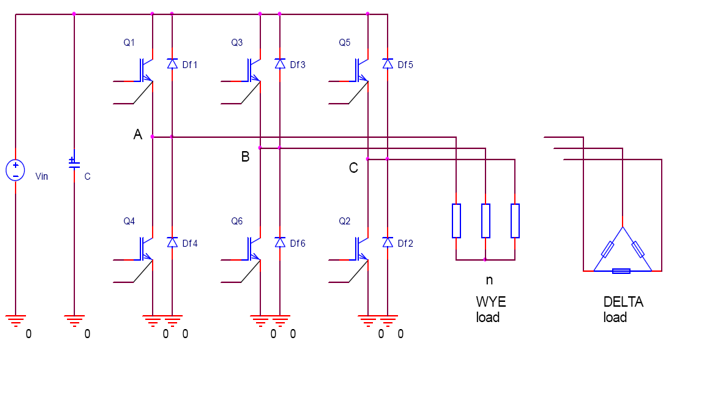
\includegraphics[width=15cm]{Imagen/inversor}
	\caption{Inversor trifásico con seis transistores con salida de tres hilos.}
	\label{fig:inversor}
\end{figure} 
 
Existen diferentes estrategias de control en inversores trifásicos (técnicas de modulación):
\begin{itemize}
	\item Modulación de 120°.
	\item Modulación de 180°.
	\item Modulación constante de ancho de pulso.
	\item Modulación senoidal de ancho de pulso (SPWM).
\end{itemize}

En la mayoría de los casos, es necesario controlar la tensión en la carga, para regular variaciones en la tensión de línea o para regular la tensión de carga.

\subsection{Modulación senoidal del ancho de pulso SPWM}
Esta técnica de modulación consigue que la THD se pueda disminuir de forma considerable. Se requieren múltiples pulsos, los cuales son generados mediante la comparación entre una tensión senoidal y una triangular. La tensión senoidal es llamada señal modulante, y de su frecuencia depende el valor de la frecuencia de la tensión de salida del inversor. Por otro lado, la tensión triangular proporciona la frecuencia de los pulsos modulados.

El índice de modulación en frecuencia se define:
\[ m_f = \frac{f_{portadora}}{f_{referencia}} = \frac{f_{triangular}}{f_{senoidal}} \]

Si $m_f$ tiene valor entero, no aparecen armónicos por debajo de la primer armónica (subarmónicos). En este caso, se dice que la modulación es SPWM síncrona, debido a que la señal triangular y la señal de control coinciden en los cruces por cero. 

Si el ídice de modulación en frecuencia no tiene un valor entero, entonces aparecerán subarmónicos que pueden ser perjudiciales para la carga, por lo que no se aconseja que la técnica SPWM sea asíncrona. Mientras mayor sea el $m_f$ mayor será el número de armónicos superiores.

Por otro lado, se puede definir el índice de modulación en amplitud como:
\[ m_a = \frac{Vmax_{referencia}}{Vmax_{portadora}} = \frac{Vmax_{senoidal}}{Vmax_{triangular}} \]

Si $0 \leq m_a \leq 1$, la amplitud de la primer armónica es proporcional a $m_a$:
\[\hat{V}_1 = ma \cdot V_{in} \]

Si $m_a \geq 1$, entonces esta relación no es proporcional, y se dice que funciona en sobremodulación, ya que en algunos instantes la señal de referencia será mayor que la triangular, por lo que la señal modulada se aproxima a una señal cuadrada. Si se sigue incrementando $m_a$, entonces el modulador se satura completamente y la señal será cuadrada. En este caso, la relación entre la amplitud de la primer armónica y la tensión de entrada es:
\[ \hat{V}_1 = \frac{4}{\pi} \cdot V_{in} \]

\section{Diseño del Inversor}
En la Fig. \ref{fig:conmutacion} se observa el circuito de potencia del inversor, encargado de llevar la potencia de entrada de CC a la carga y transformarla en potencia de CA. Las llaves controladas por tensión representan transistores de potencia. Para obtener una señal de $380$ $V_{RMS}$ es necesario suministrar una tensión continua de aproximadamente $550$ $V$. Para obtener una señal de salida con características sinusoidales se utilizan cargas inductivas.

\begin{figure}[h!]
	\centering
	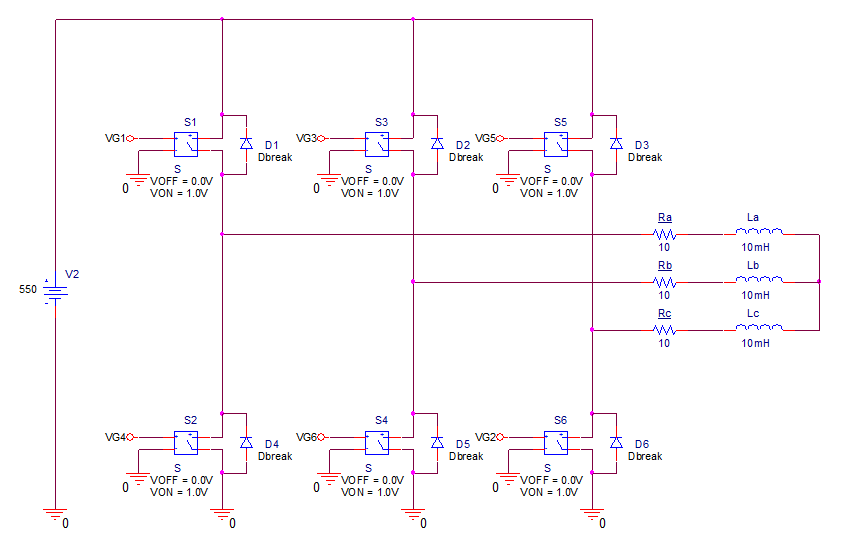
\includegraphics[width=15cm]{Imagen/Conmutacion}
	\caption{Circuito de potencia.}
	\label{fig:conmutacion}
\end{figure}

En la Fig. \ref{fig:control} se observa el circuito de control, encargado de generar el patrón de conmutación de los elementos de potencia del inversor. Este está formado por bloques matemáticos disponibles en el software de simulación, Orcad Pspice. Estos bloques representan elementos que en la práctica son comparadores analógicos y compuertas lógicas.

El primer bloque se encarga de generar la onda senoidal de amplitud $A$ y frecuencia $fm$. El segundo bloque se encarga de comparar la onda senoidal anterior con una onda triangular de frecuencia $fs$. A la salida de estos bloques se obtiene la señal de comando de los elementos de potencia de la rama superior. El último //bloque se encarga de invertir la señal proveniente de la comparación para comandar los elementos de potencia de la rama inferior del inversor.
\begin{figure}[h!]
	\centering
	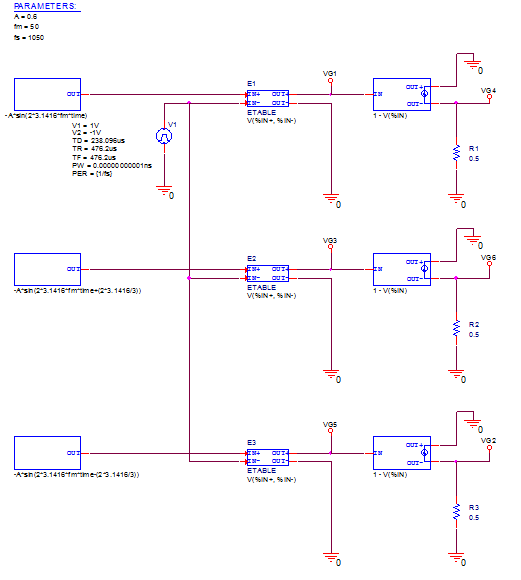
\includegraphics[width=15cm]{Imagen/Disparo}
	\caption{Circuito de control de disparo de los elementos de conmutación.}
	\label{fig:control}
\end{figure}



\newpage


\section{Simulación}
A continuación se presentan los resultados obtenidos de la simulación del circuito para distintos indices de modulación de amplitud y frecuencia.

\subsection{Señales de Control}
En la Fig. \ref{fig:VsinVtrian} se observa la señal triangular o portadora y las señales senoidales de referencia para la generación de los pulsos de mando que se observan, a su vez separada de las demas se observan los pulsos en una de las compuertas de los transistores.
 
\begin{figure}[h!]
	\centering
	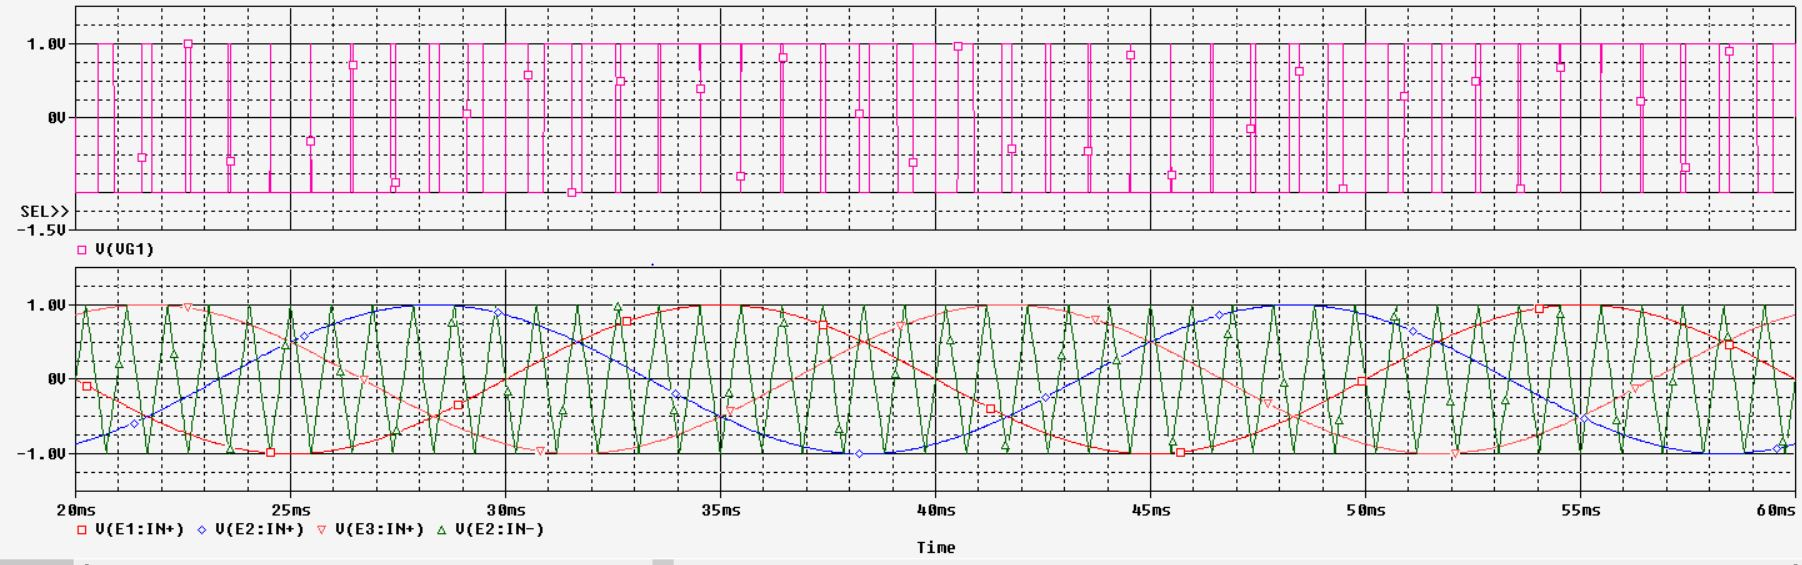
\includegraphics[width=15cm]{primer/Entrada_vs_rampa}
	\caption{Señal portadora y señales de referencia.}
	\label{fig:VsinVtrian}
\end{figure} 

\subsection{Tensión eficaz de línea y de fase, Corriente de fase}
En la Fig. \ref{fig:VabRMS} se observa la tensión eficaz de línea $Vab$ y en la Fig. \ref{fig:VanRMS} la de fase $Van$, en ambos casos para distintos indices de modulación en amplitud. Estos son: 0.25, 0.5, 0.75, 1, 1.25.

\begin{figure}[h!]
	\centering
	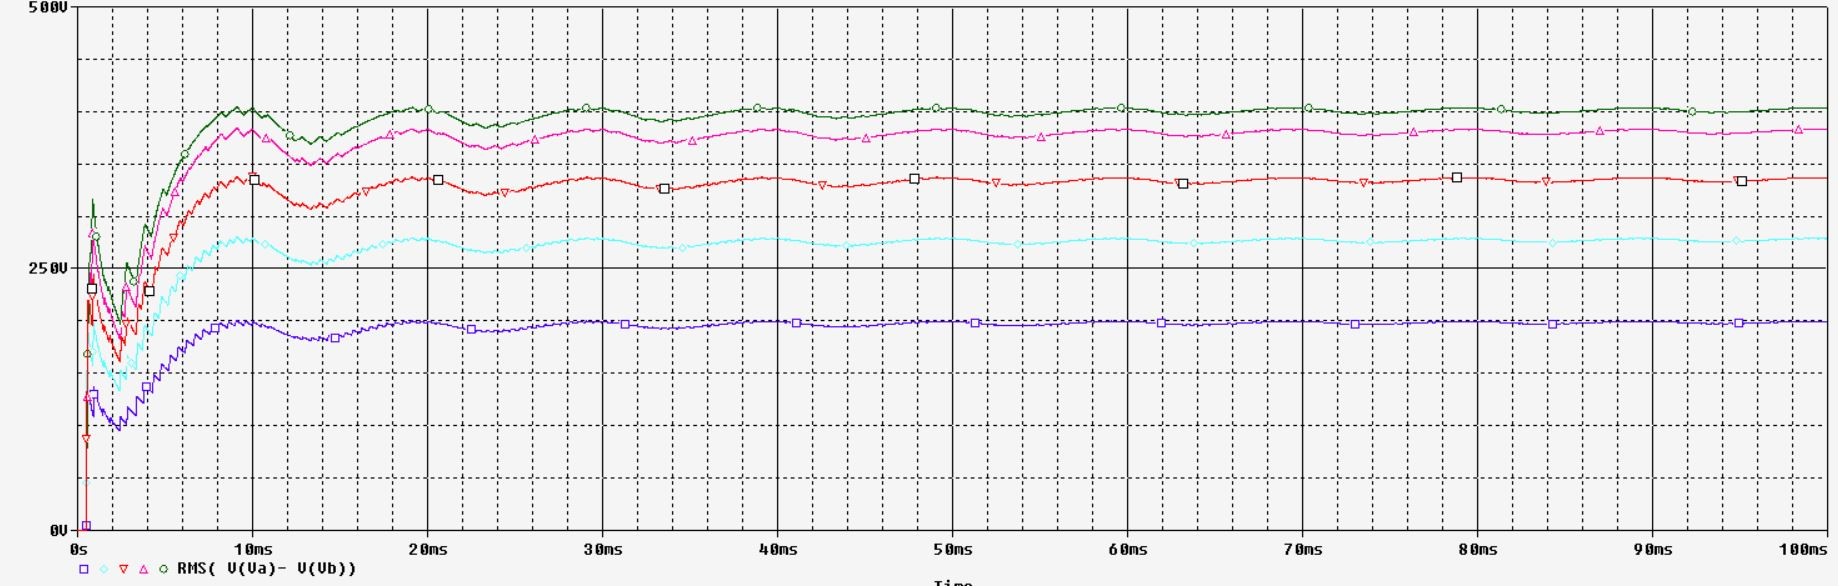
\includegraphics[width=15cm]{primer/RMSLinea}
	\caption{Tensión eficaz de línea Vab.}
	\label{fig:VabRMS}
\end{figure}

\begin{figure}[h!]
	\centering
	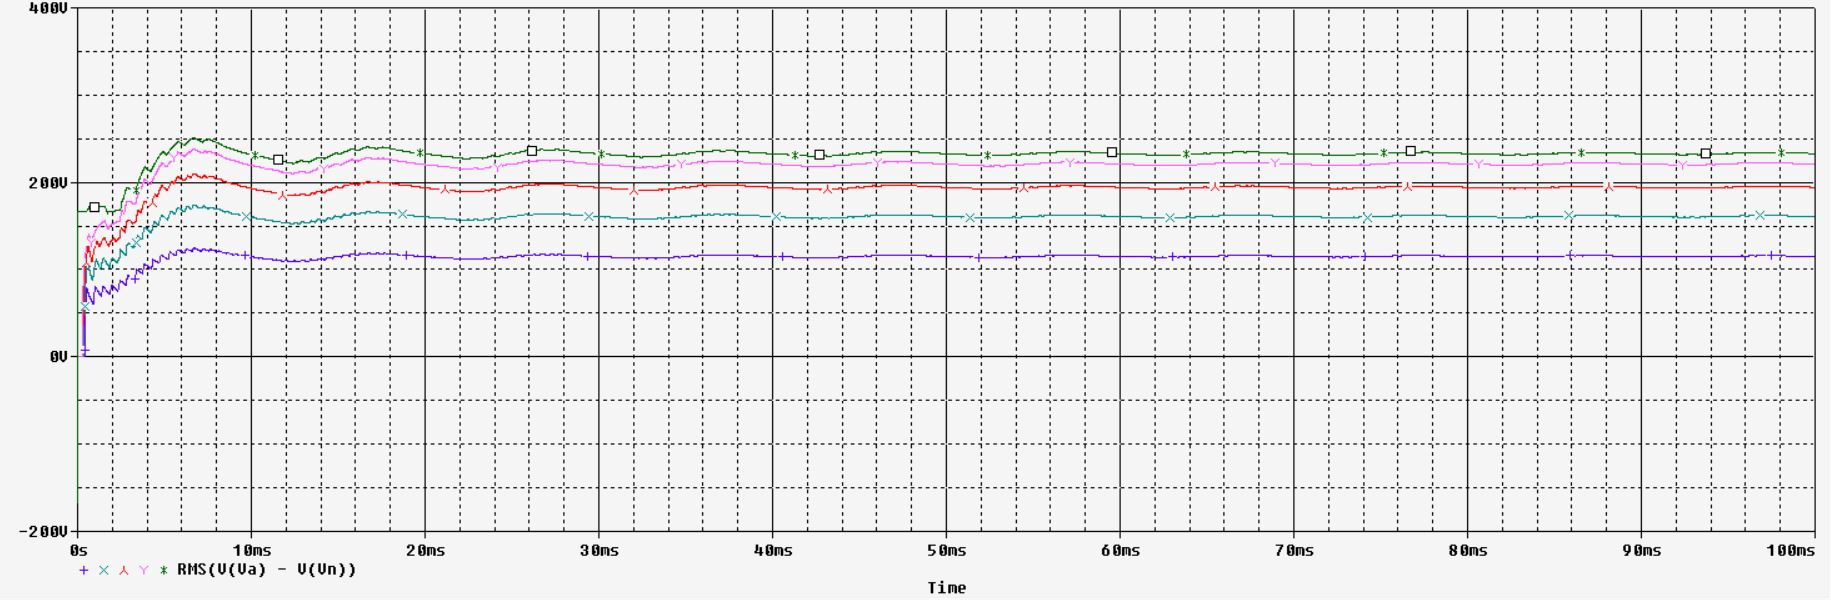
\includegraphics[width=15cm]{primer/RMSfase}
	\caption{Tensión eficaz de fase Van.}
	\label{fig:VanRMS}
\end{figure}

\newpage

En la Fig. \ref{fig:Iama} se observa como varía la corriente de fase Ia para distintos indices de modulación.

\begin{figure}[h!]
	\centering
	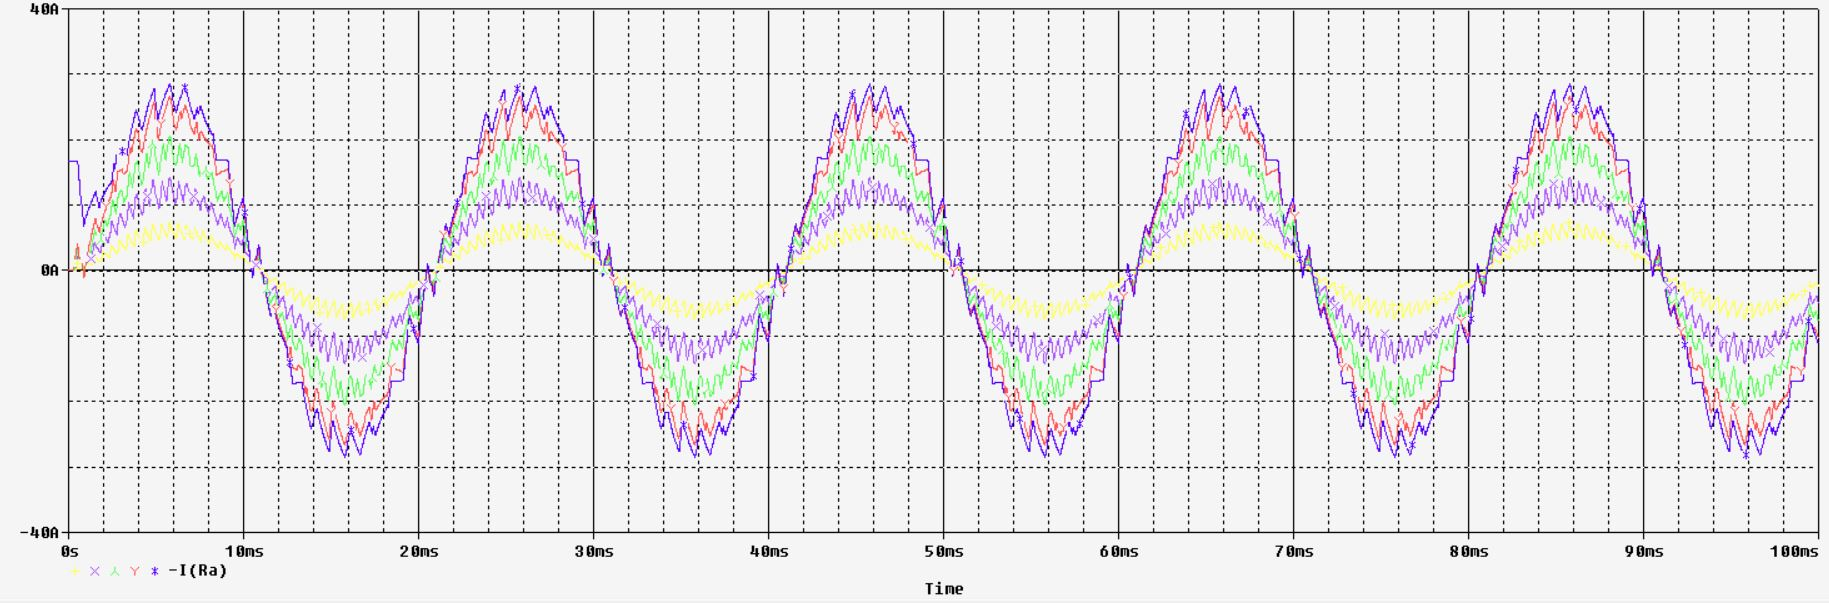
\includegraphics[width=15cm]{primer/Ifase}
	\caption{Corriente de fase Ia.}
	\label{fig:Iama}
\end{figure}

\subsection{Simulación 1}
Las señales de control utilizadas tienen las siguientes características: 
\begin{itemize}
\item $f_{triang} = 1050 \; Hz$
\item $f_{sen} = 50 \; Hz$
\item $Vmax_{triang} = 1 \;V$
\item $Vmax_{sen} = 0.6 \; V$
\end{itemize}
En este caso se tienen los siguientes índices de modulación: $mf = 21$ y $ma = 0.6$


\begin{figure}[h!]
\centering
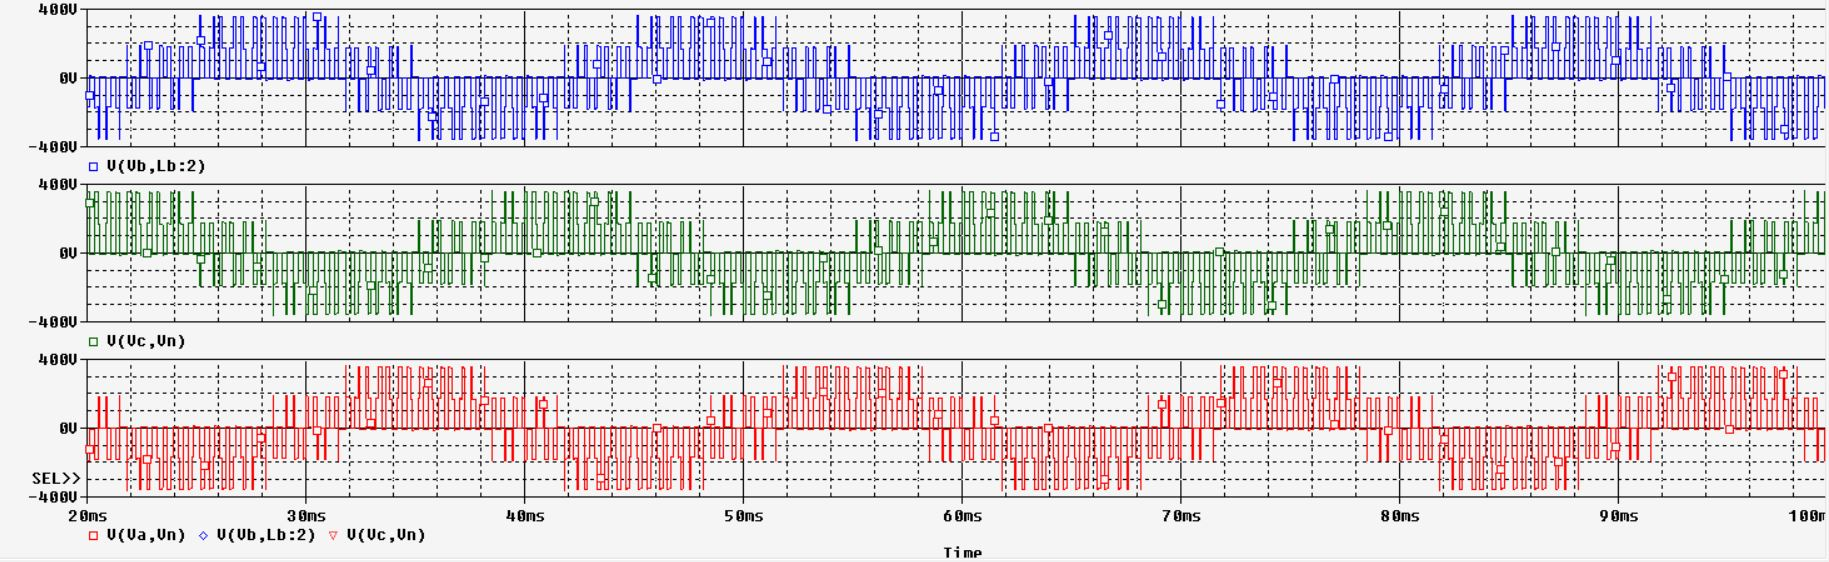
\includegraphics[width=15cm]{primer/V_Fase1mejor}
\caption{Tensiones de fase.}
\label{fig:Vfase21}
\end{figure}

\begin{figure}[h!]
\centering
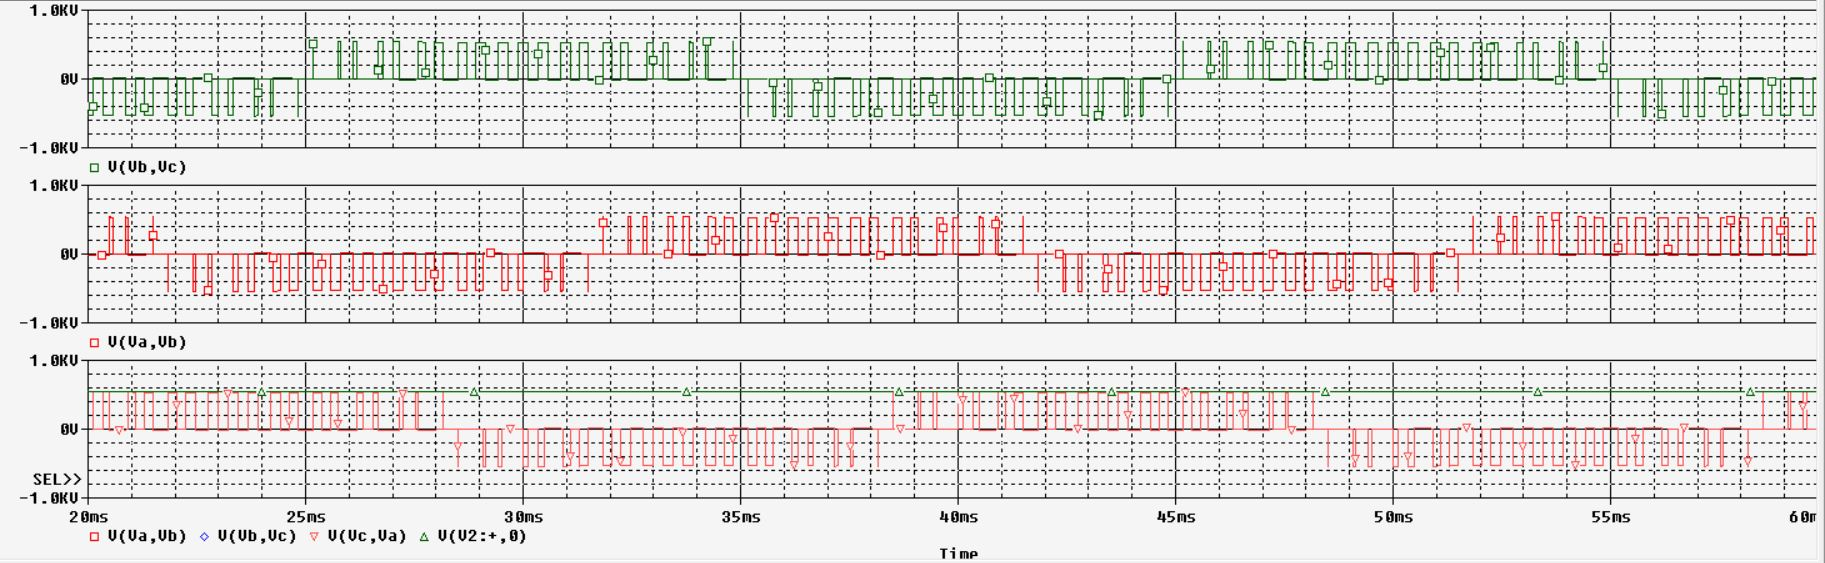
\includegraphics[width=15cm]{primer/V_Linea}
\caption{Tensiones de linea.}
\label{fig:Vlinea21}
\end{figure}

\begin{figure}[h!]
\centering
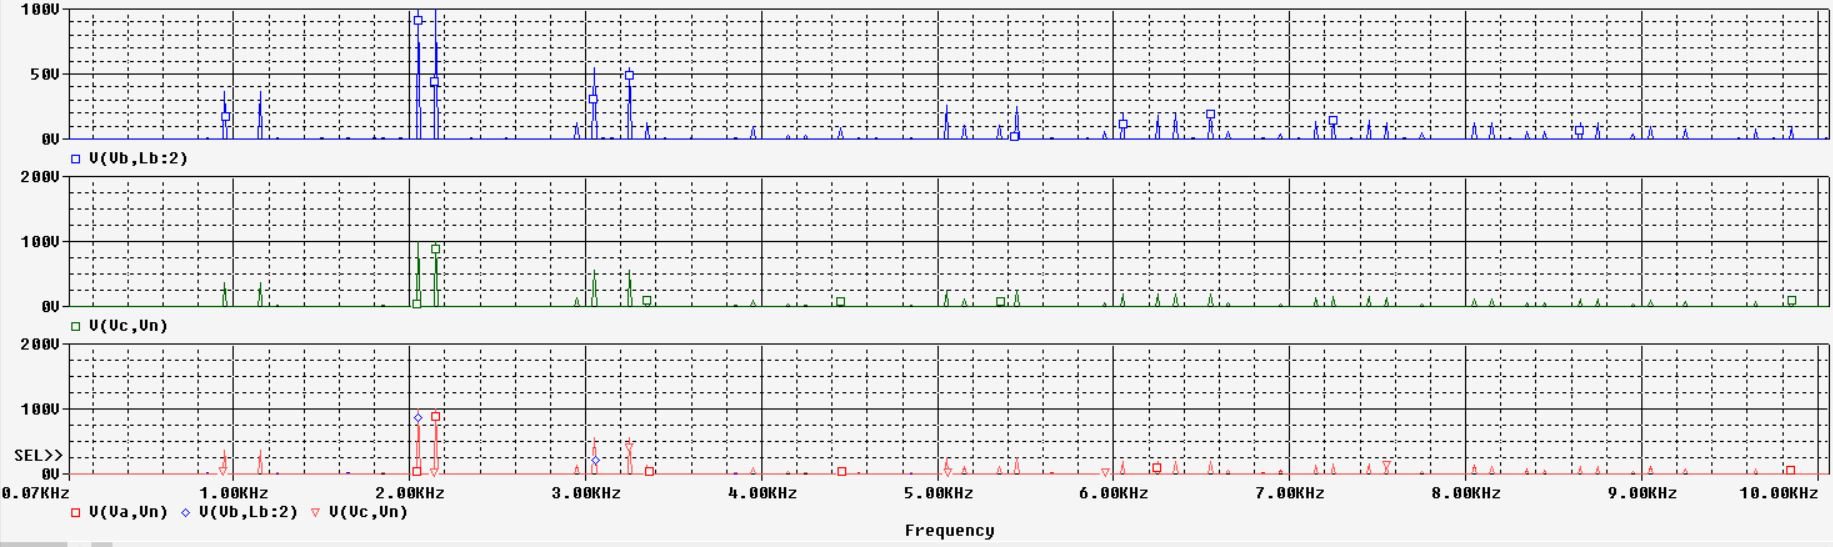
\includegraphics[width=15cm]{primer/Espectro_Fase1}
\caption{Espectro de las tensiones de fase.}
\label{fig:esp21}
\end{figure}

\newpage

\subsection{Simulación 2}
Las señales de control utilizadas tienen las siguientes características: 
\begin{itemize}
\item $f_{triang} = 1050 \; Hz$
\item $f_{sen} = 200 \; Hz$
\item $Vmax_{triang} = 1 \;V$
\item $Vmax_{sen} = 0.6 \; V$
\end{itemize}
En este caso se tienen los siguientes índices de modulación: $mf = 5.25$ y $ma = 0.6$


\begin{figure}[h!]
\centering
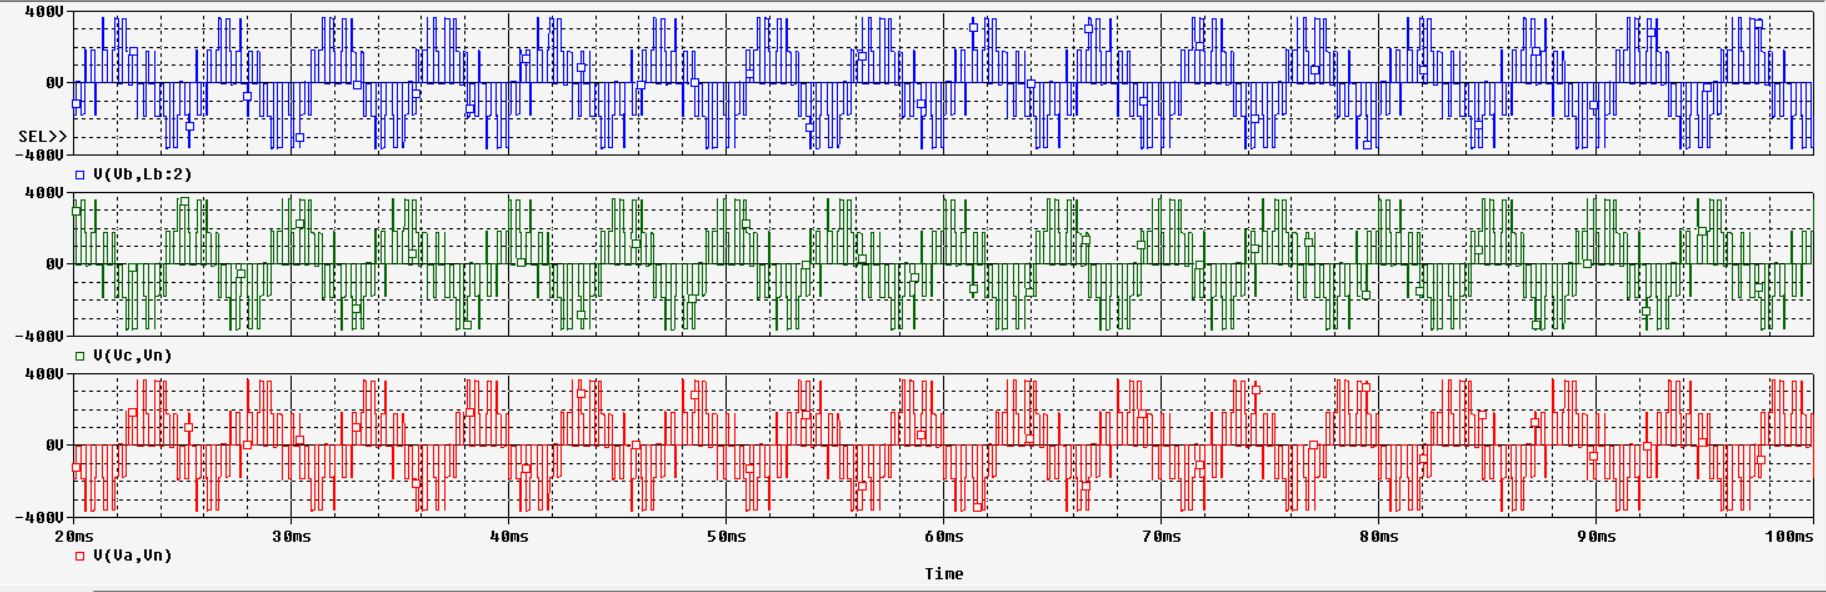
\includegraphics[width=15cm]{Segundo/Vfase}
\caption{Tensiones de fase.}
\label{fig:Vfase525}
\end{figure}

\begin{figure}[h!]
\centering
\includegraphics[width=15cm]{Segundo/vlinea}
\caption{Tensiones de linea.}
\label{fig:Vlinea525}
\end{figure}

\begin{figure}[h!]
\centering
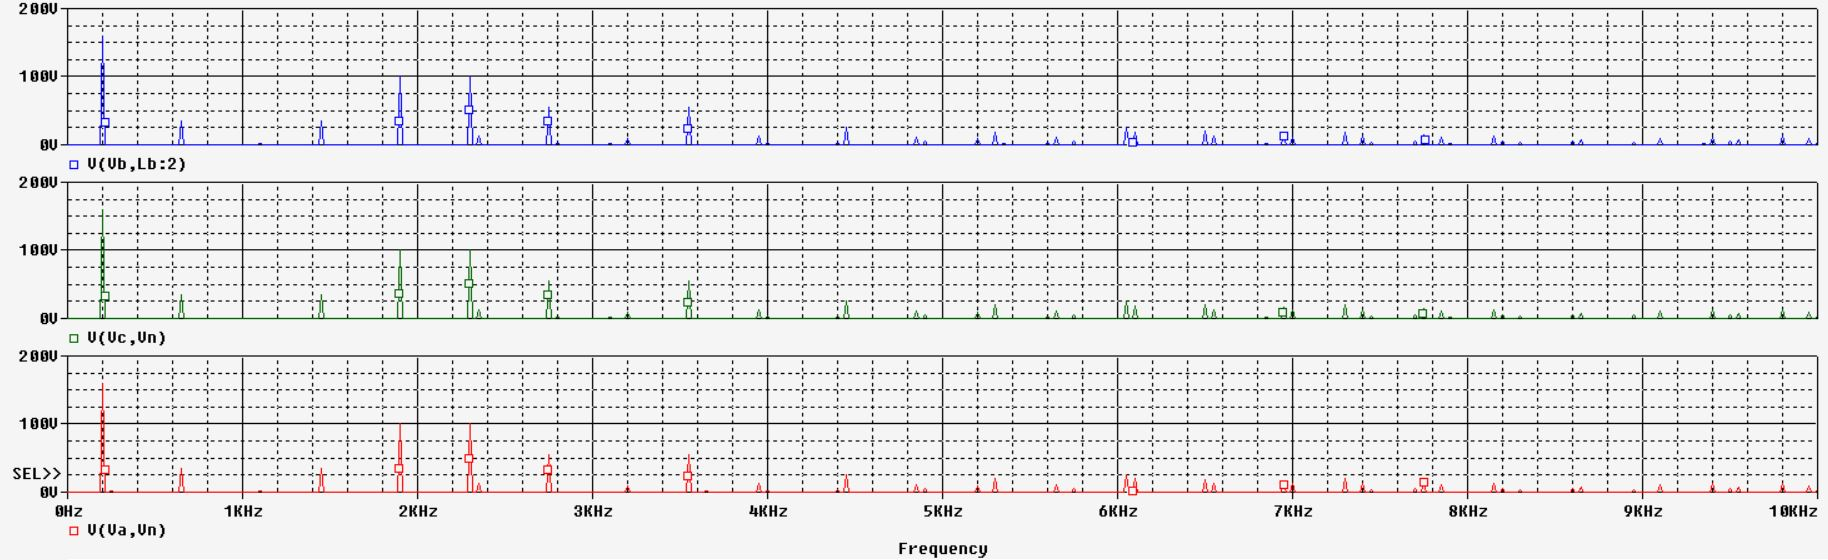
\includegraphics[width=15cm]{Segundo/Espectro}
\caption{Espectro de las tensiones de fase.}
\label{fig:esp525}
\end{figure}

\newpage

\subsection{Simulación 3}
Las señales de control utilizadas tienen las siguientes características: 
\begin{itemize}
\item $f_{triang} = 1050 \; Hz$
\item $f_{sen} = 2 \; Hz$
\item $Vmax_{triang} = 1 \;V$
\item $Vmax_{sen} = 1 \; V$
\end{itemize}
En este caso se tienen los siguientes índices de modulación: $mf = 525$ y $ma = 1$


\begin{figure}[h!]
\centering
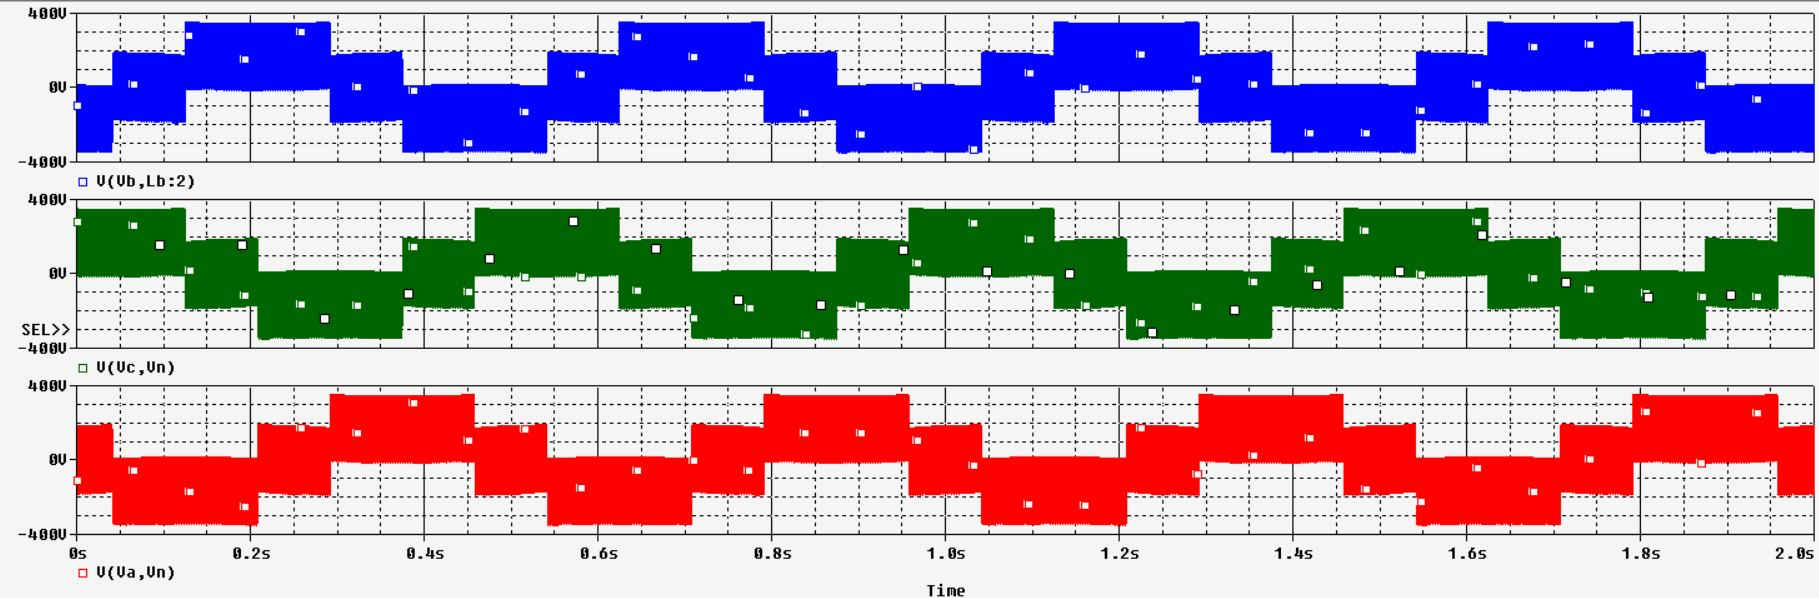
\includegraphics[width=15cm]{Tercero/Vfase}
\caption{Tensiones de fase.}
\label{fig:Vfase5.25}
\end{figure}

\begin{figure}[h!]
\centering
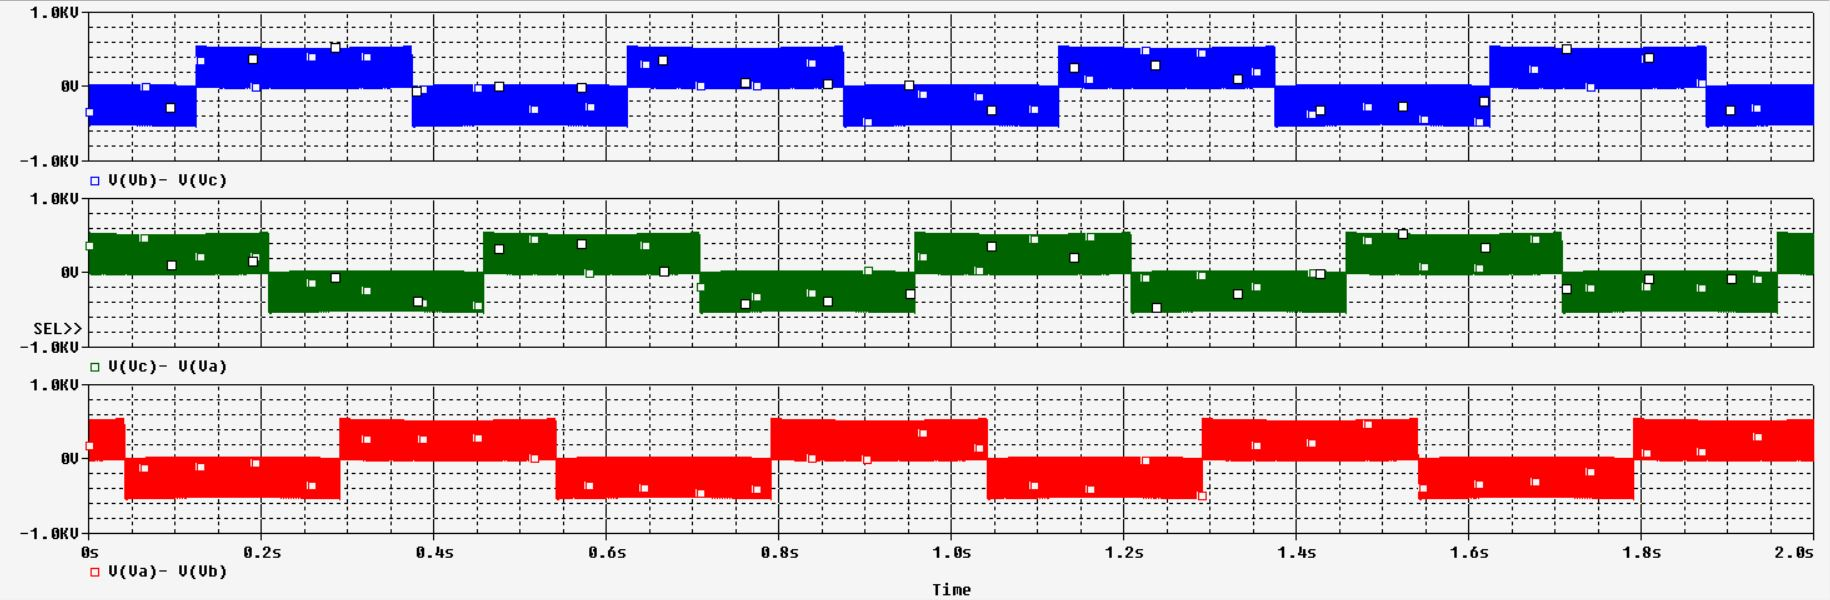
\includegraphics[width=15cm]{Tercero/Vlinea}
\caption{Tensiones de linea.}
\label{fig:Vlinea5.25}
\end{figure}

\begin{figure}[h!]
\centering
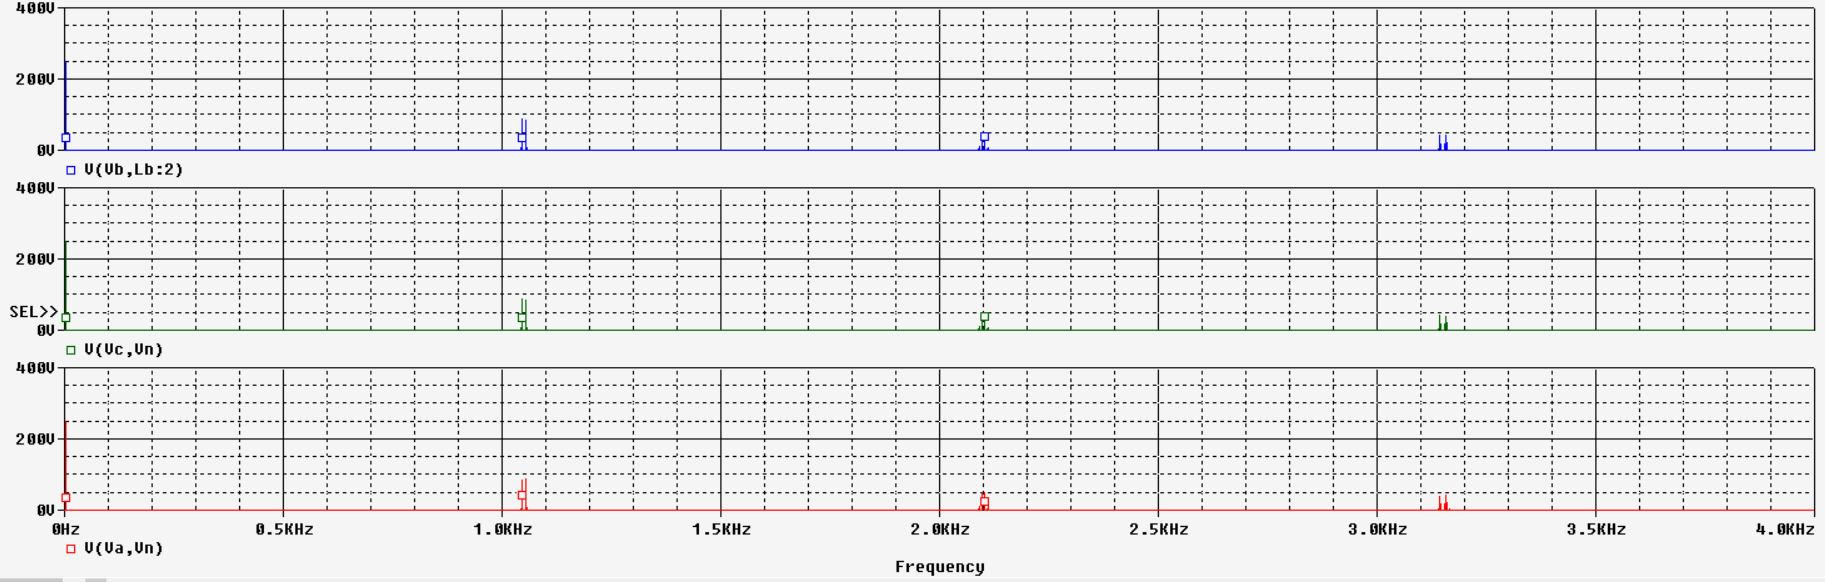
\includegraphics[width=15cm]{Tercero/Espectro}
\caption{Espectro de las tensiones de fase.}
\label{fig:esp5.25}
\end{figure}




\clearpage
\section{Conclusiones}
Respecto a la señales de control se puede decir que, la señal cuadrada se produce cuando la señal portadora y la modulante coinciden en un punto. A su vez se observa que la positividad de la señal de control depende de la portadora y no da la modulante.

Al observar las gráficas de tensión y corriente eficaz, se ve, en cualquiera de los casos, que mientras mayor sea el índice de modulación de amplitud mayor será la amplitud de la señal de salida, sea tensión o corriente. 

Se aprecia que a medida que se aumenta el $mf$ el contenido armónico disminuye, es decir, que el mejor caso de simulación es el que tiene menor frecuencia de la señal modulante, por ende, menor frecuencia de señal de salida. En este caso se produce la onda de salida mas senoidal de las tres simulaciones. Además, se facilita el filtrado de la componente fundamental, ya que el segundo armónico se encuentra distanciado de esta.

Se puede ver que la frecuencia de la señal de salida corresponde con la frecuencia de la señal modualnte (senoidal). Además se mantiene el desfasaje de la señal modulante (120°) en la señal de salida.

En todos los casos se observa que aparecen bandas laterales centradas en cada una de las armónicas de la frecuencia de portadora. Las primeras armónicas en aparecer se encuentran centradas en la frecuencia de la portadora por lo que eligiendo un mf elevado son fácilmente filtrables.

Para finalizar, la técnica SPWM aplicada a los inversores presenta diversas ventajas, ya que la señal de salida presenta una componente fundamental que depende de la frecuencia de la señal modulante, por lo que variando la frecuencia de esta se puede variar la frecuencia de la señal de salida. Además, las demás componentes en frecuencia de la señal de salida están en la frecuencia de la portadora, lo que facilita mucho el filtrado de la señal de salida, reduciendo la THD. Finalmente, es posible variar la amplitud de la señal de salida modificando el índice de modulación en amplitud

\end{document}
